%!TEX root = ../paper.tex
\begin{figure}[H]
\centering
%\textbf{Time performance means}\\[4pt]
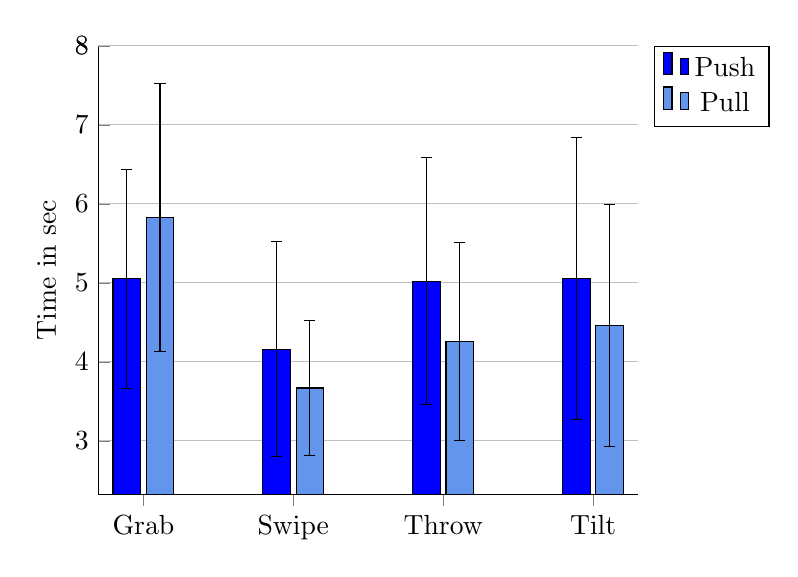
\begin{tikzpicture}
\begin{axis}[
    ybar,
    legend pos = outer north east,
    ylabel={Time in sec},
    %xlabel={Technique},
    symbolic x coords={Grab,Swipe,Throw,Tilt},
    xtick=data,
    axis lines*=left,
    ymajorgrids,
    extra y ticks=8,
    extra y tick style={grid=none},
    ytick={1,...,8}
    ]
\addplot[fill=blue] plot[error bars/.cd, y dir=both, y explicit] coordinates {
    (Grab,5.05) +- (1.385,1.385)
    (Swipe,4.16) +- (1.361,1.361) 
    (Throw,5.02) +- (1.565,1.565)
    (Tilt,5.06) +- (1.785,1.785)
    };
\addplot[fill=CornflowerBlue] plot[error bars/.cd, y dir=both, y explicit] coordinates {
    (Grab,5.83) +- (1.697,1.697)
    (Swipe,3.67) +- (0.859,0.859) 
    (Throw,4.26) +- (1.254,1.254)
    (Tilt,4.46) +- (1.532,1.532)
    };
\legend{Push,Pull}
\end{axis}
\end{tikzpicture}
\caption{The time means for each technique.}
\end{figure}

% \begin{tikzpicture}
%\pgfplotsset{symbolic x coords={Grab,Swipe,Throw,Tilt}, ymin=0, ymax=19, ybar stacked, ylabel={Time in sec}, xtick=data}
%\begin{axis}[bar shift=-8pt,
%    legend pos = outer north east, legend style = {name = serieA}, reverse legend]
%    \addplot[black, fill=CornflowerBlue, postaction={pattern=north east lines}] plot[error bars/.cd, y dir=both, y explicit] coordinates {
%    (Grab,4.81) +- (1.307,1.307)
%    (Swipe,3.83) +- (1.236,1.236) 
%    (Throw,4.72) +- (1.504,1.504)
%    (Tilt,4.66) +- (1.652,1.652)
%    };
%    \addplot[fill=CornflowerBlue] plot[error bars/.cd, y dir=both, y explicit] coordinates {
%    (Grab,5.3) +- (1.421,1.421)
%    (Swipe,4.5) +- (1.399,1.399) 
%    (Throw,5.33) +- (1.565,1.565)
%    (Tilt,5.48) +- (1.825,1.825)
%    };
%    \addplot[fill=CornflowerBlue] plot[error bars/.cd, y dir=both, y explicit] coordinates {
%    (Grab,5.05) +- (1.385,1.385)
%    (Swipe,4.16) +- (1.361,1.361) 
%    (Throw,5.02) +- (1.565,1.565)
%    (Tilt,5.06) +- (1.785,1.785)
%    };
%    \legend{Push (large), Push (small), Push (total)}
%  \end{axis}
%  \begin{axis}[bar shift = 8pt,
%  legend style = {at = {([yshift = -4.5mm, xshift = -4.5mm]serieA.south west)},
%      anchor = north west}, reverse legend]
%    \addplot[black, fill=blue, postaction={pattern=north east lines}] plot[error bars/.cd, y dir=both, y explicit] coordinates {
%    (Grab,5.46) +- (1.474,1.474)
%    (Swipe,3.42) +- (1.474,1.474) 
%    (Throw,4.02) +- (1.256,1.256)
%    (Tilt,4.18) +- (1.411,1.411)
%    };
%    \addplot[fill=blue] plot[error bars/.cd, y dir=both, y explicit] coordinates {
%    (Grab,6.19) +- (1.824,1.824)
%    (Swipe,3.92) +- (0.858,0.858) 
%    (Throw,4.51) +- (1.206,1.206)
%    (Tilt,4.76) +- (1.6,1.6)
%    };
%    \addplot[fill=CornflowerBlue] plot[error bars/.cd, y dir=both, y explicit] coordinates {
%    (Grab,5.83) +- (1.697,1.697)
%    (Swipe,3.67) +- (0.859,0.859) 
%    (Throw,4.26) +- (1.254,1.254)
%    (Tilt,4.46) +- (1.532,1.532)
%    };
%    \legend{Pull (large), Pull (small), Pull (total)}
%  \end{axis}
% \end{tikzpicture}